\documentclass[iop,numberedappendix,apj]{emulateapj}

\usepackage{epsfig}
%\usepackage{amsmath}
\usepackage{amsmath,amsthm,amssymb,cases}
\usepackage{rotating}
\usepackage{natbib}
\usepackage{enumerate}
\usepackage{multirow}
\usepackage{array}
\usepackage{appendix}
\usepackage{comment}
\usepackage{color,xcolor}
\usepackage{url}
\usepackage{ulem}
\usepackage{here}
\usepackage{hyperref}
\hypersetup{colorlinks,linkcolor={blue!50!black},citecolor={blue!50!black},urlcolor={blue!50!black}}
\allowdisplaybreaks[1]
\bibliographystyle{apj}
\renewcommand{\bibname}{References}

\def\plotonesc#1{\centering \leavevmode
\includegraphics[clip=, width=1.70\columnwidth]{#1}}
\def\plotoneh#1{\centering \leavevmode
\includegraphics[clip=, width=.95\columnwidth]{#1}}
\def\plotone#1{\centering \leavevmode
\includegraphics[clip=, width=.85\columnwidth]{#1}}
\def\plotoneShrinkSmall#1{\centering \leavevmode
\includegraphics[clip=, width=.49\columnwidth]{#1}}
\def\plotoneShrinkMed#1{\centering \leavevmode
\includegraphics[clip=, width=.55\columnwidth]{#1}}
\def\plotoneShrinkBig#1{\centering \leavevmode
\includegraphics[clip=, width=.65\columnwidth]{#1}}
\def\plottwo#1#2{\centering \leavevmode
\includegraphics[width=.45\columnwidth]{#1} \hfil
\includegraphics[width=.45\columnwidth]{#2}}
\def\plottwob#1#2{\centering \leavevmode
\includegraphics[width=.49\columnwidth]{#1} \hfil
\includegraphics[width=.49\columnwidth]{#2}}
\def\plottwor#1#2{\centering \leavevmode
\includegraphics[width=.55\columnwidth,angle=90]{#1} \hfil
\includegraphics[width=.55\columnwidth,angle=90]{#2}}
\def\plotthree#1#2#3{\centering \leavevmode
\includegraphics[width=.3\columnwidth]{#1} \hfil
\includegraphics[width=.3\columnwidth]{#2} \hfil
\includegraphics[width=.3\columnwidth]{#3}}

\def\gsim{\;\rlap{\lower 2.5pt
 \hbox{$\sim$}}\raise 1.5pt\hbox{$>$}\;}
\def\lsim{\;\rlap{\lower 2.5pt
   \hbox{$\sim$}}\raise 1.5pt\hbox{$<$}\;}
%\def\fast{\;$f^{\ast }$\;}
\def\fast{\tilde f}

% set formatting properties
\setlength{\textwidth}{6.5in}
\setlength{\textheight}{8.8in}
\setlength{\hoffset}{0.0in}
\setlength{\voffset}{-0.4in}
\parindent 0.2in
\parskip 0.1in

\def\edit#1{\textcolor{red}{#1}}
\def\memoYF#1{\color{red}[YF: {\bf #1}]\color{black}}
\def\memoJLY#1{\color{green}[JLY: {\bf #1}]\color{black}}
\def\memoNBC#1{\color{blue}[NBC: {\bf #1}]\color{black}}



%%% http://www.oceanwave.jp/index.php?float%B4%C4%B6%AD(figure%2Ftable)%A4%CE%BD%D0%CE%CF%B0%CC%C3%D6%A4%F2%A5%B3%A5%F3%A5%C8%A5%ED%A1%BC%A5%EB

%%%%%%%%%%%%%%%%%%%%%%%%%%%%%%%%%%%%%%%%%%%%%%%%%
% THE DOCUMENT BEGINS HERE                      %
%%%%%%%%%%%%%%%%%%%%%%%%%%%%%%%%%%%%%%%%%%%%%%%%%

%\slugcomment{Submitted to ApJ, XX September 2015}

\begin{document}

\title{Rotational Spectral Unmixing of Exoplanets:\\Degeneracies between Surface Colors and Geography}


\author{
%
Yuka Fujii\altaffilmark{1,2} 
%
Jacob Lustig-Yaeger\altaffilmark{3,4,5} 
%
Nicolas B. Cowan\altaffilmark{6,7} 
%
}

\affil{$^1$NASA Goddard Institute for Space Studies, 
  New York, NY 10025, USA}
      
\affil{$^2$Earth-Life Science Institute, Tokyo Institute of Technology, 
  Tokyo, 152-8550, JAPAN}
  
\affil{$^3$Astronomy Department, University of Washington, Box 951580, Seattle, WA 98195, USA}

\affil{$^4$Astrobiology Program, University of Washington, 3910 15th Ave. NE, Box 351580, Seattle, WA 98195, USA}

\affil{$^5$NASA Astrobiology Institute -- Virtual Planetary Laboratory Lead Team, USA}

\affil{$^6$Department of Earth and Planetary Sciences, McGill University, Montreal, Quebec
Canada H3A 0E8}

\affil{$^7$Department of Physics, McGill University, Montreal, Quebec
Canada H3A 0E8}



\vspace{0.5\baselineskip}

\email{
yuka.fujii.ebihara@gmail.com
}

\begin{abstract}

Unmixing the disk-integrated spectra of exoplanets provides a clue to \edit{heterogeneous surfaces} that we cannot directly resolve in the foreseeable future. 
It is particularly important for terrestrial planets with diverse surface compositions like Earth. 
Although previous work on unmixing the spectra of Earth from disk-integrated multi-band light curves appeared successful, we \edit{point out} a mathematical degeneracy between the surface colors and their spatial  distributions. 
Nevertheless, \edit{useful constraints on the spectral shape of individual surface types may be obtained from the fact that albedo should be between 0 to 1, depending on the trajectory of the planet in color space}.  
We demonstrate the degeneracy and the possible constraints using both the mock data based on a toy model of Earth and the observed data of Earth. 
Despite the severe degeneracy, we are still able to recover an approximate albedo spectra for ocean. 
\edit{We find that observing at multiple wavelengths where surfaces albedo is close to 0 or 1 will provide better constraints. }

\end{abstract}

\keywords{planets and satellites: surfaces --- planets and satellites: terrestrial planets}
  
%]%%% End front material



%%%%%%%%%%%%%%%%%%%%%%%%%%%%%%%%%%%%%%%%%%%%%%%%%%%%%%%%%%%%%%%%%%%
\section{Introduction}
\label{sec:intro}
%%%%%%%%%%%%%%%%%%%%%%%%%%%%%%%%%%%%%%%%%%%%%%%%%%%%%%%%%%%%%%%%%%%

Direct imaging of exoplanets is expected to play a vital role in characterizing Earth analogs in habitable zones and beyond. 
Substantial work has gone into prediciting detectable features in disk-integrated spectra of Earth and other planets, as they are observed from an astronomical distance. 
\edit{Disk-integrated spectra or even multi-band photometry (colors) in principle include the effects of the surface reflectance as well as the atmosphere. (We use the term spectra and colors interchangeably.) }
%Atmospheric molecules are identifiable through spectral absorption features \citep[e.g.,][]{DesMarais2002} but surface reflectance spectra also affect the spectra, which could be measured through low-resolution spectra, or multi-band photometry. 
However, interpreting disk-integrated colors is not trivial. 
This is particularly true for Earth-like planets that harbor diverse atmospheric and surface characteristics including liquid water, partial cloud cover, continents, and possibly vegetation. 

A key here is to leverage the time variation of the spectrum\edit{/color}  \citep{Ford2001}: the regions that contributes to the scattered light change due to the planetary rotation and  orbital motion, so \edit{the time variability can be used to map the} heterogeneity of the surface environment.  
\citet{Cowan2009, Cowan2011} performed Principal Component Analysis (PCA) on the observed multi-band photometry of Earth. They found that the number of surface types can be inferred from the number of dominant principle components: (\# of surface types) $\ge $ (\# of principal components) $+ 1$. %) and that the variation pattern is indicative of the surface properties. 
\citet{Fujii2010, Fujii2011} decomposed multi-band photometric data of the Earth assuming the template reflectance spectra of the known major surface types, and they found that the relative abundance and the longitudinal variation of these surface types are approximately recovered. 
Moreover, by coupling the time variation due to rotation with phase variation due to orbital revolution, a 2-dimensional map of the surface may be retrieved \citep{Kawahara2010, Kawahara2011, Fujii2012}. 

\citet{Cowan2013} took another approach to the same inverse problem. 
Their strategy was to try to estimate the reflectance spectra of surfaces and their geographical maps across the globe simultaneously, by making all of them fitting parameters. 
They applied their method to the light curves of the Earth observed \edit{by} EPOXI, and the result appeared successful in so far as they obtained reflectance spectra roughly matching the average spectra of clouds, ocean, and continents. 
However, the longitudinal map of these components did not match the actual geography.  

We are motivated by this unsatisfactory result to revisit their analysis. 
We start by creating mock light curves to see if we can fully retrieve the known answer. 
Taking a close look at the mathematical relation between the colors and geographical maps of the surfaces, we discuss the degeneracy among them. 
We then demonstrate using the mock data how our estimate are constrained given the physical conditions, including the expectation that albedo should be between 0 and 1. 
\edit{We also apply the same procedure to the data observed by EPOXI. }

The organization of this paper is as follows. 
In Section \ref{s:mockdata}, we introduce our toy-model multi-band diurnal light curves of Earth. 
\edit{Section \ref{s:frame} analyzes the mock data, with the description of general framework to approach this problem. } 
In Section \ref{s:EPOXI}, we apply our procedure to the EPOXI light curves and attempt to estimate the surface colors of the Earth. 
Section \ref{s:discussion} discusses the possible improvements on our estimation as well as a few confounding factors, including the degeneracy between the planetary albedo and the planetary radius. 
Finally Section \ref{s:conclusion} concludes the paper. 

%%%%%%%%%%%%%%%%%%%%%%%%%%%%%%%%%%%
\begin{figure}[h]
    \begin{center}
	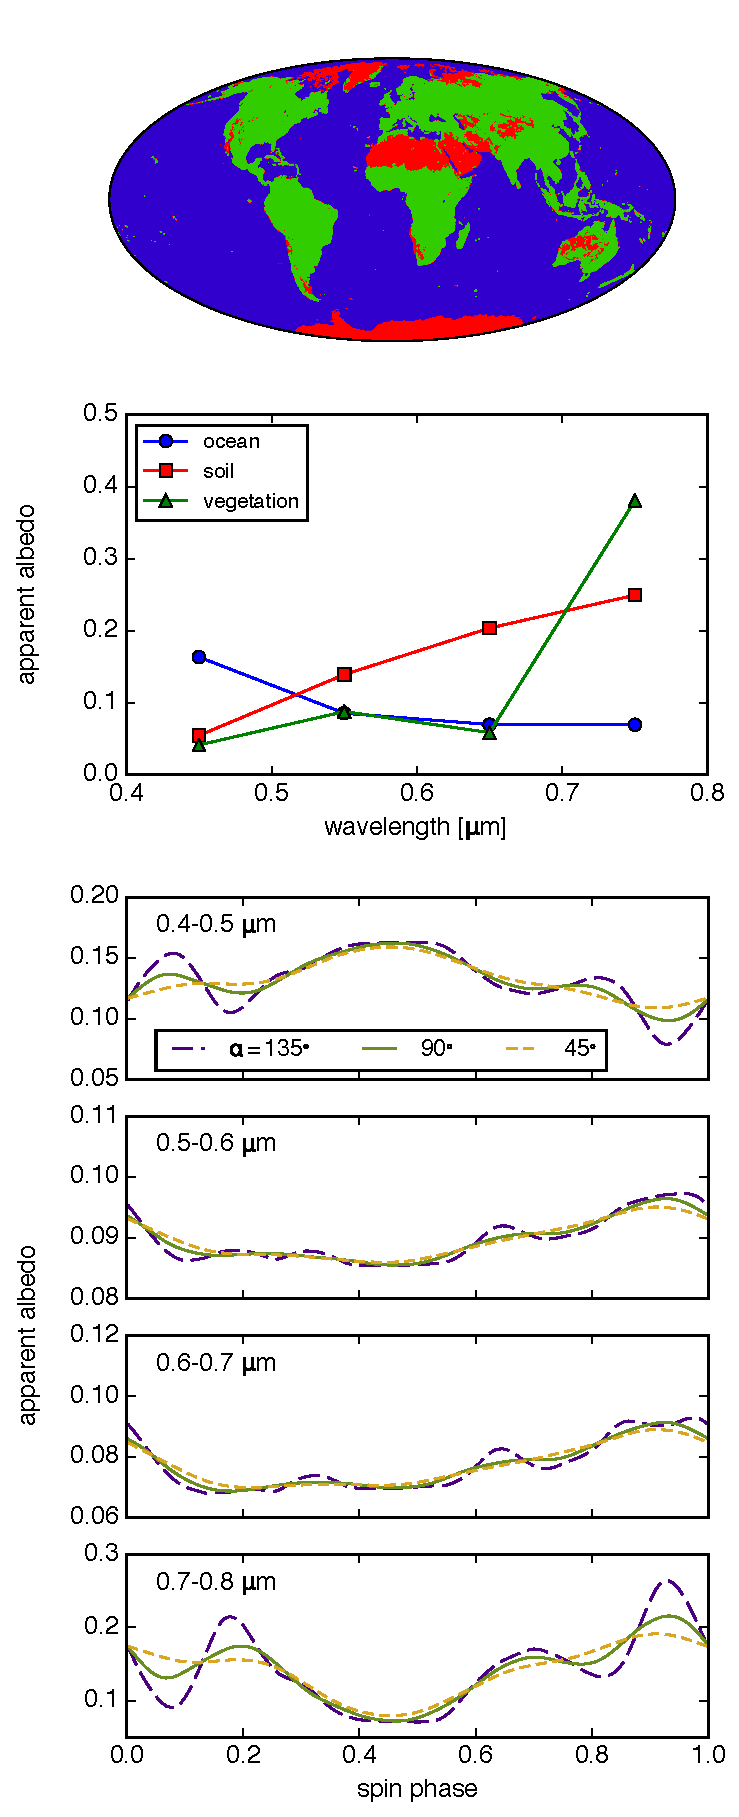
\includegraphics[width=\hsize]{mockdata.pdf}
    \end{center}
    \caption{Our mock data based on IGBP classification map of the Earth. Top panel: distribution of 3 surface types (ocean: blue, sand: red, vegetation: green). Middle panel: assumed albedo spectra with matching colors. Bottom 4 panels: rotational light curves in 4 photometric band with varying phase angle, $\alpha = 135^{\circ }$ (purple, dot-dashed), $90^{\circ }$ (olive, solid), and $45^{\circ }$ (gold, dashed). }
\label{fig:mockdata}
\end{figure}
%%%%%%%%%%%%%%%%%%%%%%%%%%%%%%%%%%%


%%%%%%%%%%%%%%%%%%%%%%%%%%%%%%%%%%%%%%%%%%%%%%%%%%%%%%%%%%%%%%%%%%%
\section{Preparing Mock Datasets}
\label{s:mockdata}
%%%%%%%%%%%%%%%%%%%%%%%%%%%%%%%%%%%%%%%%%%%%%%%%%%%%%%%%%%%%%%%%%%%

In order to facilitate the discussions in the following sections, we shall introduce a mock dataset to be used for demonstrations in this section. 

We consider diurnal light curves of a toy model of the atmosphere-less Earth, in 4 photometric bands. 
We use a simplified surface map as shown in the upper left panel of Figure \ref{fig:mockdata}. 
This map is based on the land classification by the International Geosphere-Biosphere Programme (IGBP)\footnote{\url{https://climatedataguide.ucar.edu/climate-data/ceres-igbp-land-classification}}. 
Although the original classification assumes 16 land surface types plus ocean, in this paper we adopt 3 surface types for simplicity regarding ``Open Shrubs'', ``Urban'', ``Snow/Ice'', and ``Barren/Desert'' as ``sand'' (red in the upper left panel of Figure \ref{fig:mockdata}) and other land surface types as ``vegetation'' (green), while keeping the ``ocean'' regions. 


The assumed albedo spectra of these surface types in 4 photometric bands are shown in the upper right panel of Figure \ref{fig:mockdata}. 
These 4 photometric bands correspond to 0.4--0.5 $\mu $m, 0.5--0.6 $\mu $m, 0.6--0.7 $\mu $m, and 0.7--0.8 $\mu $m, respectively, but we will simply refer to them by the band indices unless otherwise noted. 
%\memoJLY{I think it would be helpful to make the "band \#"-axis wavelength in microns, and then perhaps refer to the band \# in the text or in an upper x-axis. }
The albedo spectrum for ocean is based on \citet{Mclinden1997}, 
and the data for \edit{sand} and vegetation are taken from ASTER spectral library\footnote{\url{https://speclib.jpl.nasa.gov/}. 
Specifically, we adopt  ``Brown to dark brown sand'' for ``\edit{sand}'', and ``Grass'' for the ``vegetation''}. 
The scattering phase function by the surface is assumed to obey the Lambert law, i.e., the radiance is (incident flux)$\times $(albedo)/$\pi$, independent of the direction of the scattering. 
Note that in reality they are not Lambertian scatterers; among others,  scattering by the ocean is particularly anisotropic at crescent phase (see Section \ref{ss:deviate_Lambert}).  

% and the albedo spectra of ocean overlaid with atmosphere  
%\memoJLY{A phase of 135 deg is right in the range that Ty (Robinson et al. 2010; 2011) shows will deviate most from a Lambertian scatterer due the ocean glint...}

%{\color{red} 
The diurnal light curves are synthesized given the relative positions of the star, planet, and observer. 
% We consider light curves of 1 rotation at a fixed orbital phases. 
For the sake of simplicity, we consider a planet with zero obliquity in an edge-on orbit, and change the phase angle (the planet-centric angle between the star and the observer) denoted by $\alpha $. 
We also assume that spin period is significantly shorter than the orbital period and the orbital phase does not change in a single spin rotation. 
However, the following discussion does not depend on these assumptions. 
We consider noise-free data. Clearly, noise in real observations of Earth twins are expected to be substantial, and the effect of such observations will be discussed elsewhere. 
%\color{black}

The bottom panels of Figure \ref{fig:mockdata} display examples of diurnal light curves in 4 photometric bands, represented in terms of {\it apparent albedo}. 
Apparent albedo is the albedo of the planet weighted by illumination and visibility. 
More specifically, it is obtained by normalizing the planetary intensity by that of a loss-less Lambert sphere with the same radius and at the same phase \citep{Qiu2003, Seager2010}. 
In this paper we will use apparent albedo unless otherwise noted. 
The apparent albedo is straightforwardly obtained from the observed planetary intensity, if and only if the planetary radius and the observational geometry are completely known: orbital phase of the planet, and the distance between the star and the planet. 

The problem throughout this paper is, from these kinds of multi-band diurnal light curves, how and how well we can retrieve the albedo spectra of different surface types and the longitudinal distribution of these surface types. 


%%%%%%%%%%%%%%%%%%%%%%%%%%%%%%%%%%%%%%%%%%%%%%%%%%%%%%%%%%%%%%%%%%%
\section{Inverse problem}
\label{s:frame}
%%%%%%%%%%%%%%%%%%%%%%%%%%%%%%%%%%%%%%%%%%%%%%%%%%%%%%%%%%%%%%%%%%%

In this section, we discuss the general framework for analying the diurnal light curves, and present some demonstrations using the mock data created in the previous section. 
Sections \ref{ss:model} and \ref{ss:PCplane} are essentially the recapitulation of previous papers, in particular \citet{Cowan2013} \citep[but see also][]{Cowan2009,Cowan2011,Fujii2010,Fujii2011}.  
We choose to include these discussions, however, as a baseline to establish the later arguments. 

%%%%%%%%%%%%%%%%%%%%%%%%%%%%%%%%%%%%%%%%%%%%%%%%%%%%%%%%%%%%%%
\subsection{Algebraic Formulation}
\label{ss:model}
%%%%%%%%%%%%%%%%%%%%%%%%%%%%%%%%%%%%%%%%%%%%%%%%%%%%%%%%%%%%%%


%%%%%%%%%%%%%%%%%%%%%%%%%%%%%%%%%%%
\begin{table}[b]
\caption{Indexes}
\begin{center}
\begin{tabular}{lcc} \hline \hline
Name & Symbol & Maximum \\ \hline
Observation Time & $i$ & I \\
Band & $j$ & J  \\
Surface Type & $k$ & K  \\
Longitudinal Slice  & $l$ & L \\ 
Principal Components & $n$ & N \\ \hline
\end{tabular}
\end{center}
\label{tab:index}
\end{table}%
%%%%%%%%%%%%%%%%%%%%%%%%%%%%%%%%%%%


Assuming that the planetary surface is everywhere Lambertian scatterering, and that it is composed of a certain number $K$ of spectrally distinct surface types, the disk-integrated scattered light is a weighted summation of the reflectance spectra of different surface types. 
Using the local surface albedo $s_{\vec \Omega }$, the zenith angle of the insolation, $\theta _0$, and the zenith angle of the observer $\theta _1$ (both defined at each surface point),
the apparent albedo of the planet \edit{in band $j$ at epoch $i$}, $d_{ij}$ (``$d$'' for data) is written as follows \citep[see][]{Fujii2010}: 
%%%
\begin{eqnarray}
d_{i} (\lambda_j) &=& \displaystyle \frac{ \int_{{\rm IV}_i} s_{\vec \Omega }(\lambda_j) \cdot \cos \theta_0 ({\vec \Omega}) \cdot \cos \theta_1 ({\vec \Omega}) \cdot d\vec \Omega }{ \int_{{\rm IV}_i}  \cos \theta_0 ({\vec \Omega}) \cdot \cos \theta_1 ({\vec \Omega}) \cdot d\vec \Omega } \\
&=& \sum _{k} s_k (\lambda_j) \; \displaystyle \frac{ \int_{{\rm IV}_{i}} f_k (\vec \Omega ) \cos \theta_0 ({\vec \Omega}) \cdot \cos \theta_1 ({\vec \Omega}) \cdot d\vec \Omega }{ \int_{{\rm IV}_i}  \cos \theta_0 ({\vec \Omega}) \cdot \cos \theta_1 ({\vec \Omega}) \cdot d\vec \Omega } \notag \\
&=& \sum _{i,k} \fast_{ik} \, s_{kj} \label{eq:tilde_d_f_ast_s}
\end{eqnarray}
%%%
where the \edit{spectrum of $k$-th surface type is represented by:}
%%%
\begin{equation}
s _{kj} \equiv  s_k (\lambda _j)
\end{equation}
%%%
and the apparent covering fraction \edit{of $k$-th surface type at epoch $i$ is}:
%%%
\begin{equation}
\tilde f_{ik} \equiv  \frac{ \int_{{\rm IV}_{i}} f_k (\vec \Omega ) \cos \theta_0 ({\vec \Omega}) \cdot \cos \theta_1 ({\vec \Omega}) \cdot d\vec \Omega }{ \int_{{\rm IV}_i}  \cos \theta_0 ({\vec \Omega}) \cdot \cos \theta_1 ({\vec \Omega}) \cdot d\vec \Omega }
\end{equation}
%%%
% and $i$, $j$, and $k$ are indices for the observation epochs, bands, and the surface types, respectively, 
\edit{where} ${\rm IV }_i$ denotes the illuminated and visible area over the planetary surface at \edit{epoch $i$}, and $f_k (\vec \Omega )$ is the area fraction of $k$-th surface type in $d\vec \Omega$. 
%In the last expression, $\fast_{ik}$ represents the apparent covering fraction of the $k$-th surface type at $i$-th observational epoch, and 
%$s_{kj}$ is the reflectance spectra of the $k$-th surface type in the $j$-th band. 
The maximum value of $i$, $j$ and $k$ will be denoted by $I$, $J$, and $K$, below, as summarized in Table \ref{tab:index}. 

By definition, the area fractions, $\fast $, should not be negative and they should sum up to unity, and reflectance spectra, $s$, should be between 0 and 1. 
Therefore, the constraints on geography ($\fast_{ik}$) and colors ($s_{kj}$) of the surfaces are:
%%%
\begin{subnumcases}
{}
0 \leq \fast_{lk} \;\;\; & \mbox{for any $l$, $k$} \label{eq:tilde_f_range} \\
\sum_k \fast_{lk} = 1 & \mbox{for any $l$} \label{eq:tilde_f_sum} \\
0 \leq s_{kj} \leq 1 \;\;\; & \mbox{for any $k$, $j$} \label{eq:tilde_s_range} 
\end{subnumcases}
%%%


%%%
%\begin{eqnarray}
%\begin{cases}
%\;\; 0 \leq s_{kj} \leq 1 \;\;\; & \mbox{for any $k$, $j$} \\
%\;\; 0 \leq \fast_{lk} \leq 1 \;\;\; & \mbox{for any $l$, $k$} \label{eq:cond_f_ast}\\
%\;\; \sum_k \fast_{lk} = 1 & \mbox{for any $l$} 
%\end{cases}
%\end{eqnarray}
%%%

%\subsection{Estimating the Composition\\of Longitudinal Slices}

The time variability of the apparent covering fraction $\fast $ due to the planet's rotation is related to the surface inhomogeneity along the equator. Approximately, $\fast _{ik}$ may be written as the weighted summation of the area fraction of the $k$-th surface type in each of longitudinal slices, i.e.,
%%%
\begin{eqnarray}
\fast _{ik} &=& \frac{ \int_{{\rm IV}_i} f_k (\vec \Omega ) \cos \theta_0 ({\vec \Omega}) \cdot \cos \theta_1 ({\vec \Omega}) \cdot d\vec \Omega }{ \int_{{\rm IV}_i}  \cos \theta_0 ({\vec \Omega}) \cdot \cos \theta_1 ({\vec \Omega}) \cdot d\vec \Omega }  \\
&=& \sum_l \frac{ \int f_k (\vec \Omega ) W_i (\vec \Omega  ) \cdot d\vec \Omega }{ \int  W_i (\vec \Omega ) \cdot d\vec \Omega } \\
%&\approx & \sum_l f_{lk} \frac{ \int W_i (\vec \Omega ) \cdot d\vec \Omega }{ \int  W_i (\vec \Omega ) \cdot d\vec \Omega } \label{eq:discretize}\\
&\approx & \sum_l  W_{il} f_{lk} \label{eq:Wf}, \\
W_{il} &\equiv & \frac{ \int  W_i (\vec \Omega  ) \cdot d\vec \Omega_l }{ \int W_i (\vec \Omega )  \cdot d\vec \Omega }
\end{eqnarray}
%%%
where $l$ is the index for longitudinal slices, $f_{lk}$ is the area fraction of the $k$-th surface type in the $l$-th longitudinal slice. 
Strictly speaking, the approximation is valid only when $f_k(\vec \Omega)$ does not change or changes little across the $l$-th slice for all $k$ and $l$. 
In the last equation, $W_{il}$ is the weight of the $l$-th longitudinal slice at epoch $i$, which depends only on the observational geometry. 
\citet{Cowan2013} refer to this as the convolution kernel, $K$. 
% As a result,

One can \edit{therefore} recast Equation (\ref{eq:tilde_d_f_ast_s}) in terms of the longitudinal map:
%%%
\begin{equation}
d_{ij} \approx \sum _{l,k} W_{il} \, f_{lk} \, s_{kj} \label{eq:d_f_s}
\end{equation}
%%%
where $f_{lk}$ is the average area fraction of $k$-th surface type at $l$-th longitudinal slice, Again, the area fractions at longitudinal slices, $f_{lk}$, cannot be negative and should sum up to unity. Thus, a set of condition similar to Equations (\ref{eq:tilde_s_range})-(\ref{eq:tilde_f_sum}) are imposed:
%%%
\begin{subnumcases}
{}
0 \leq f_{lk} \;\;\; & \mbox{for any $l$, $k$} \label{eq:f_range} \\
\sum_k f_{lk} = 1 & \mbox{for any $l$} \label{eq:f_sum} \\
0 \leq s_{kj} \leq 1 \;\;\; & \mbox{for any $k$, $j$} \label{eq:s_range}
\end{subnumcases}
%%%
Now, the relevant problem is, given $d$, estimate $\{f, s\}$ subject to the constraints of Equations (\ref{eq:s_range})-(\ref{eq:f_sum})---this is where \citet{Cowan2013} stood. 
In principle, constraints (\ref{eq:f_sum}) and (\ref{eq:s_range}) are more stringent than (\ref{eq:tilde_f_sum}) and (\ref{eq:tilde_s_range}), due to the low-pass filter nature of the map-to-lightcurve convolution. 


%%%%%%%%%%%%%%%%%%%%%%%%%%%%%%%%%%%
\begin{figure}[b!]
    \begin{center}
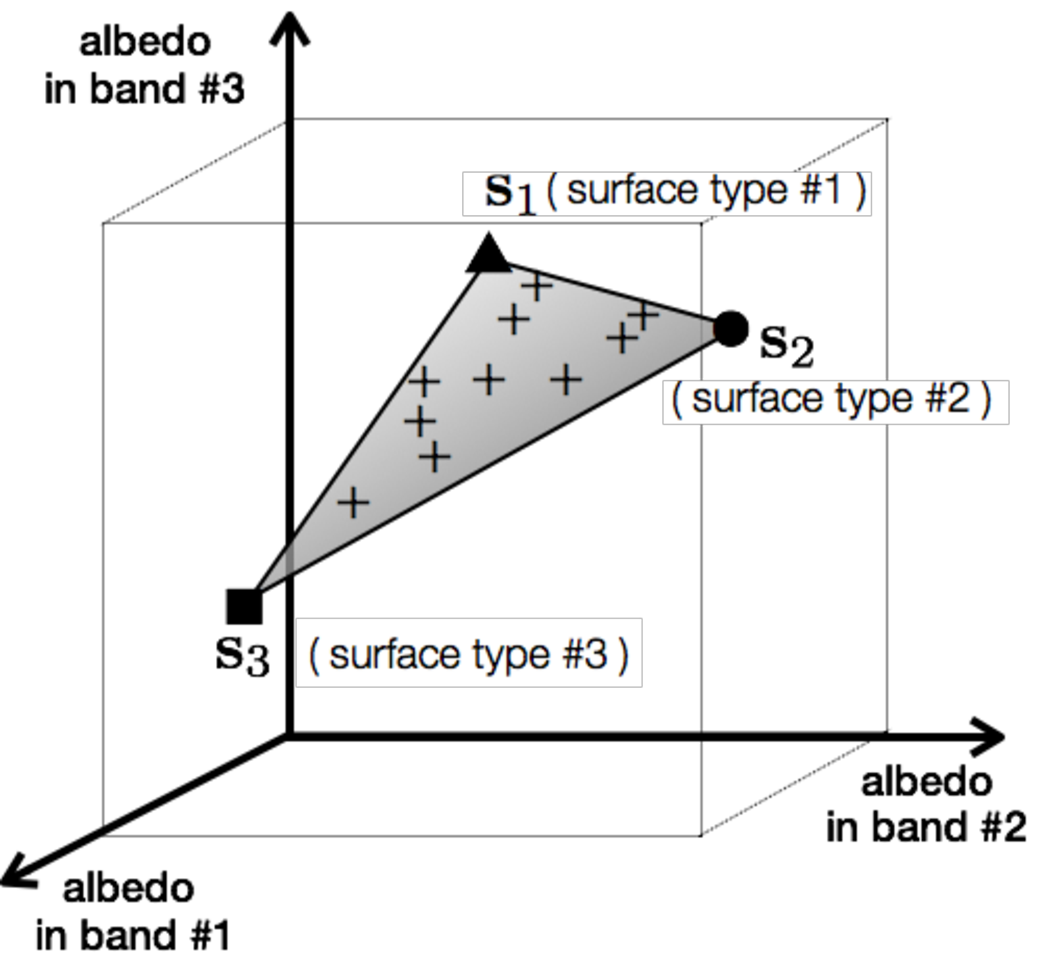
\includegraphics[width=0.8\hsize]{schematics_ver3.pdf}
    \end{center}
    \caption{\edit{Schematic figure to illustrate the relation between observed data ($\{{\bf d}_i\} $; crosses) and surface spectra ($\{{\bf s}_k\} $; filled points). The dashed cube shows the range where physical albedo can exist (between 0 and 1). }}
\label{fig:schematic}
\end{figure}
%%%%%%%%%%%%%%%%%%%%%%%%%%%%%%%%%%%


%%%%%%%%%%%%%%%%%%%%%%%%%%%%%%%%%%%%%%%%%%%%%%%%%%%%%%%%%%%%%%
\subsection{Graphical Conception on \\Principal Component Plane}
\label{ss:PCplane}
%%%%%%%%%%%%%%%%%%%%%%%%%%%%%%%%%%%%%%%%%%%%%%%%%%%%%%%%%%%%%%

%A question is whether the above formulation leads us to a unique solution of either $\{ {\bf \fast},\,{\bf s} \}$ or $\{ {\bf f},\,{\bf s}\}$, given the data matrix, ${\bf d}$. 

Equation (\ref{eq:tilde_d_f_ast_s}) coupled with the conditions (\ref{eq:tilde_f_range}) and (\ref{eq:tilde_f_sum}) indicates a geometrical relationship among ${\bf d}$, ${\bf \fast }$, and ${\bf s}$ in 
$J$-dimensional space, where $\{{\bf d}_i\}$ are located on the plane defined by $K$ surfaces, $\{{\bf s}_k\} $, and in the region enclosed by $\{{\bf s}_k\} $. 
%\memoYF{How is it called in one word in mathematics?}
Figure \ref{fig:schematic} graphically shows this relations in the case of $J=3$ and $K=3$. 
Note that the dimension of this plane is $K-1$, so in general it is a hyper-plane.  
%We show this graphically in Figure \ref{fig:trajectory}, using the mock datasets shown in Section \ref{s:mockdata}. 

This plane can be identified by performing Principal Component Analysis (PCA) \citep{Cowan2009,Cowan2011}, as PCA extracts the major, mutually-orthogonal axes along which the data are scattered. 
Consequently, the number of major principal components (PCs) are equal to or less than $K-1$ \citep{Cowan2011}. 
Note that non-Lambertian reflectance, partially transparent cloud cover, or observational noise would in practice ensure that the PC plane has some thickness (see also Section \ref{ss:deviate_Lambert}). 

From the mock light curves prepared in Section \ref{s:mockdata}, 
we use PCA to extract two dominant principal components (PCs) through PCA with other components having virtually zero contributions, consistent with the 3 input surface types.  
The PCs extracted from the light curves at $\alpha = 90^{\circ }$ (olive lines in Figure \ref{fig:mockdata}) are presented in the upper panel of Figure \ref{fig:trajectory}. 
For later use, we denote these PCs by $V_{nj}$ where $n=1$ or $2$  corresponding to the 1st and 2nd PC. 
Since we use the same three surface spectra throughout, the principal component plane is the same in all cases, but the individual PCs may be rotated. 

\edit{Using $V_{nj}$ and the time average of the colors in the case of $\alpha = 90^{\circ }$, $\bar d_j$, the light curves are projected onto the PC plane by}:
%%%
\begin{equation}
d_{ij} = \sum_n U_{in} V_{nj} + \bar d_j
\end{equation}
%%%
where $U_{in}$ is the trajectory. %\edit{\sout{The $V_{nj}$) and the time-averaged colors ($\bar d_j$) uniquely specify the PC plane. }
% in the PC plane and $\bar d_j$ is the time average of the colors. % as the offset. 
\edit{The trajectory of the light curves at different orbital phases are shown by the olive line in Figure \ref{fig:trajectory}. }
%\edit{\sout{The dominant PCs ($V_{nj}$) and the time-averaged colors ($\bar d_j$) uniquely specify the PC plane. }}
%We may plot the trajectories of other light curves at different phase angles on the same plane because the PC plane should be the same\edit{\sout{ plane regardless of orbital phase}}. %(under the noiseless condition) because we use the same 3 surface types and assume Lambertian surfaces. 
% (Note that PCA on individual light curves does not necessarily find the same PCs, because it depends on how the data points are scattered on the PC plane.)
%Thus, the trajectories of the mock light curves at different phase angles are also shown in the lower panel of Figure \ref{fig:trajectory}. 
The color excursions are greater at a larger phase angle (crescent phase), because less surface area is averaged together.  
The points in the figure indicate the input albedo spectra of the three surface types. 
As described above, the trajectories are always inside the triangle defined by these points. 
%Because the apparent albedo at any time of the observations is a linear combination of input surface colors (Equation \ref{eq:tilde_d_f_ast_s}) under the conditions (\ref{eq:tilde_f_range}) and (\ref{eq:tilde_f_sum}), the trajectories should always be inside the triangle defined by these points.  
 
%%%%%%%%%%%%%%%%%%%%%%%%%%%%%%%%%%%
%\begin{figure}[tbh!]
%    \begin{center}
%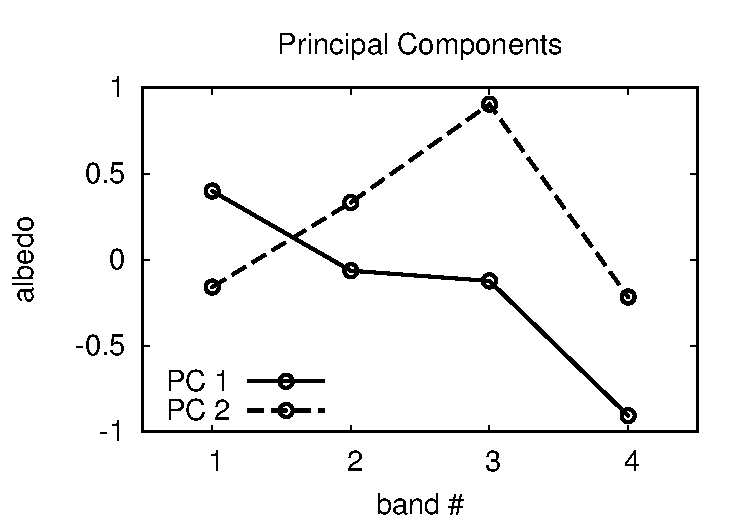
\includegraphics[width=\hsize]{PCA_V_jn.pdf}
%    \end{center}
%    \caption{Principal components of the light curves shown in the bottom of Figure \ref{fig:mockdata}. }
%\label{fig:PCs}
%\end{figure}
%%%%%%%%%%%%%%%%%%%%%%%%%%%%%%%%%%%

%%%%%%%%%%%%%%%%%%%%%%%%%%%%%%%%%%%
\begin{figure}[t]
    \begin{center}
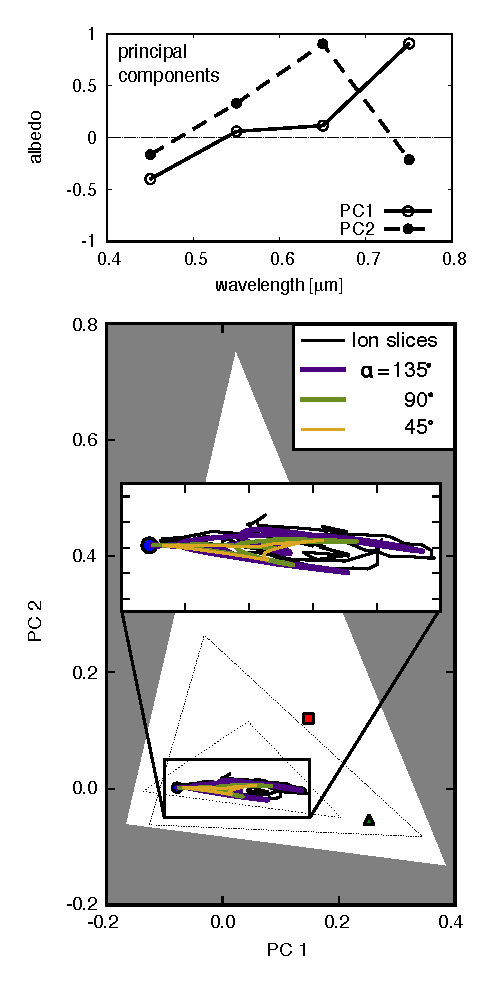
\includegraphics[width=\hsize]{mockdata_PCplane.pdf}
    \end{center}
    \caption{Upper panel: principal components of the light curves at $\alpha = 90^{\circ }$ shown in olive lines in Figure \ref{fig:mockdata}. Lower panel: trajectories of the 4-band light curves on the PC plane set by 2 PCs shown in the upper panel, in the case of $\alpha = 135^{\circ }$ (indigo thick line), $\alpha = 90^{\circ }$ (olive line), and $\alpha = 45^{\circ }$ (gold thin line). Points indicate the input albedo spectra of ocean (blue circle), \edit{sand} (red square), and vegetation (green triangle) on the PC plane. Points in the gray region violate the condition (\ref{eq:tilde_s_range}); specifically, the left, right, and bottom boundaries are set by $s_{k,4} > 0$, $s_{k,1} > 0$, and $s_{k,3}> 0$, respectively. 
Dotted lines are random triangle that could be solutions (see text). }
    \label{fig:trajectory}
\end{figure}
%%%%%%%%%%%%%%%%%%%%%%%%%%%%%%%%%%%

%%%%%%%%%%%%%%%%%%%%%%%%%%%%%%%%%%%%%%%%%%%%%%%%%%%%%%%%%%%%%%
\subsection{\edit{Degenerate Solutions}}
\label{ss:degeneracy}
%%%%%%%%%%%%%%%%%%%%%%%%%%%%%%%%%%%%%%%%%%%%%%%%%%%%%%%%%%%%%%

When it comes to the inverse problem of estiamting the surface spectra given the trajectory/-ies, {\it any} set of $\{ {\bf s}_k \}$ that enclose the data points $\{{\bf d}_i\}$ in the principal component plane can be a solution of Equation (\ref{eq:tilde_d_f_ast_s}) subject to the conditions (\ref{eq:tilde_f_range}) and (\ref{eq:tilde_f_sum}). 
Two such example are shown by the dotted lines in Figure \ref{fig:trajectory}. 
Note that the associated matrix, $\fast _{ik}$, can always be found. 

Additional constraints come from the condition (\ref{eq:tilde_s_range}). 
In Figure \ref{fig:trajectory} any points in the shadowed region are rejected based on this condition: specifically, the left, right, and bottom boundaries are set by $s_{k,4}> 0$, $s_{k,1}> 0$, and $s_{k,3}> 0$. 
In other words, surface lying in the forbidden gray regions have negative albedo. 
While in this particular example the permitted region happens to be a triangle, shape can differ depending on the location of the principal component plane relative to the albedo boundaries. 
Since each of 4 bands has lower and upper bounds on albedo, $0<s<1$, the physically allowed region of color space is a 4-dimensional hypercube, also known as tesseract. Depending on the orientation of the PC plane with this tesseract, the allowed region may have a variety of geometries. 
In general, the allowed region is a $K-1$ dimensional slice through a $J$-dimensional hypercube. 

%Although this is not sufficient to result in a unique solution, it does impact the precision of rotational spectral unmixing as discussed below. 

In Figure \ref{fig:trajectory} we show two random triangles that enclose the trajectory; these triangles satisfy the conditions (\ref{eq:tilde_f_range}) and (\ref{eq:tilde_f_sum}), as do many others. 
For example, with a large triangle one can have spectrally interesting surface spectra and boring geography (small longitudinal variation in area fractions) while with a small triangle one can have boring surface spectra (different surfaces look similar) and interesting geography. 
Therefore, predicting ${\bf \fast }$ and ${\bf s}$ from ${\bf d}$ is degenerate.  

A formally equivalent degeneracy is found in Equation (\ref{eq:d_f_s}) coupled with the conditions (\ref{eq:f_range})-(\ref{eq:s_range}). 
Essentially, the term $\sum _k f_{lk} s_{kj}$ represents the average albedo spectra of $l$-th slice and $W_{il}$ is the matrix that convolve them into the light curves. 
Suppose idealistically that we can retrieve the average spectra of longitudinal slices from the light curves through $W_{il}$; the black trajectory in the bottom panel of Figure \ref{fig:trajectory} represents the color variation as a function of longitude.  
We again have different sets of $\{ {\bf s}_k \}$ that enclose the averaged albedo spectra of longitudinal slices {\it and} are located in the range of condition (\ref{eq:s_range}). 
%, any of which can make up the given averaged albedo spectra with the associated $f_{lk}$. 
Nevertheless, the excursions of the longitudinal colors are more dramatic than the disk-integrated colors of the light curves, thus the possible solutions are somewhat restricted. 
% For disk-integrated light curves, the color excursions are more muted than the intrinsic longitudinal map, so the degeneracy becomes severer. 


%%%%%%%%%%%%%%%%%%%%%%%%%%%%%%%%%%%%%%%%%%%%%%%%%%%%%%%%%%%%%%
\subsection{``Best Guess'' of the Surface Types}
\label{ss:guess}
%%%%%%%%%%%%%%%%%%%%%%%%%%%%%%%%%%%%%%%%%%%%%%%%%%%%%%%%%%%%%%


%%%%%%%%%%%%%%%%%%%%%%%%%%%%%%%%%%%
\begin{figure*}[tbh!]
   \begin{minipage}{0.33\hsize}
    \begin{center}
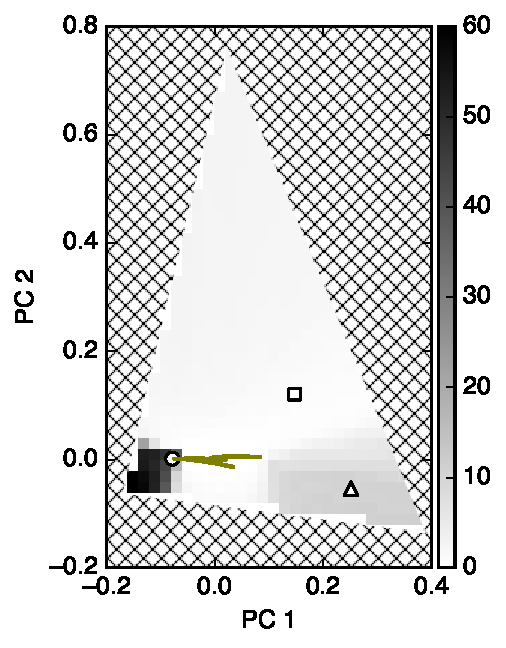
\includegraphics[width=\hsize]{mockdata_90deg_3types_t360_lc_noreg_allowedregion_gray.pdf}
%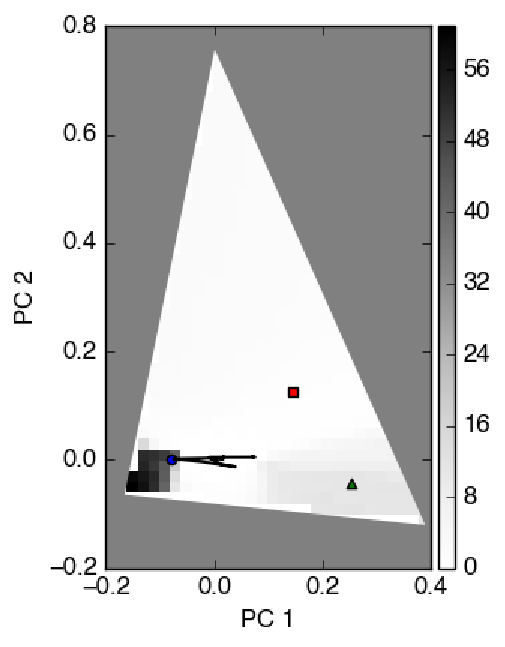
\includegraphics[width=\hsize]{mockdata_90deg_3types_t12_lc_noreg.pdf}
    \end{center}
     \end{minipage}   
    \begin{minipage}{0.33\hsize}
    \begin{center}
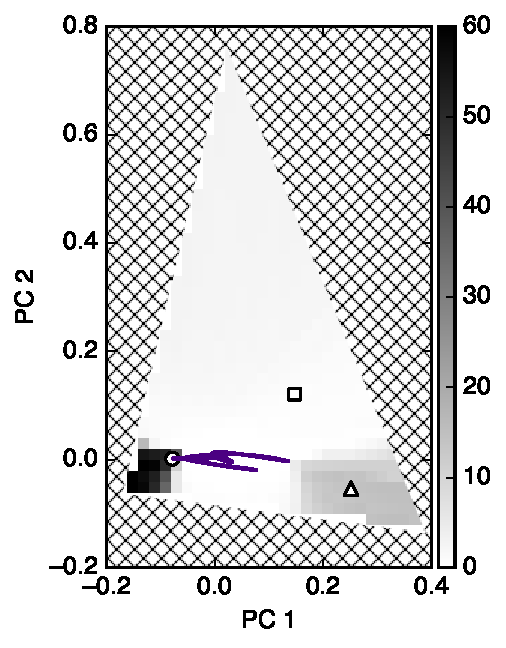
\includegraphics[width=\hsize]{mockdata_135deg_3types_t360_lc_noreg_allowedregion_gray.pdf}
%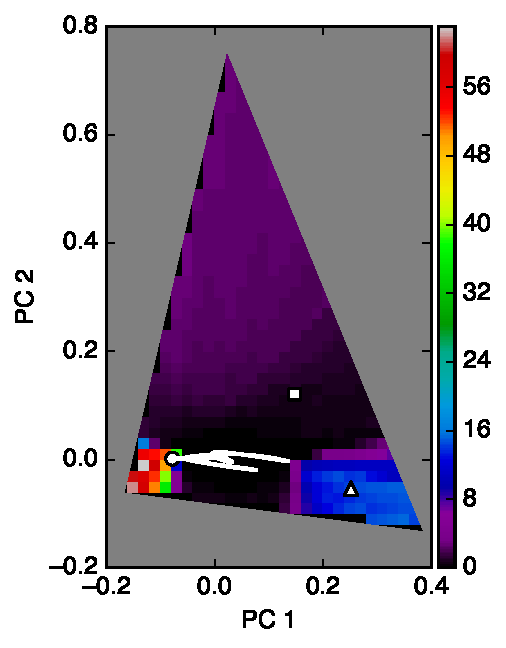
\includegraphics[width=\hsize]{mockdata_135deg_3types_t360_lc_noreg.pdf}
    \end{center}
     \end{minipage}
   \begin{minipage}{0.33\hsize}
    \begin{center}
%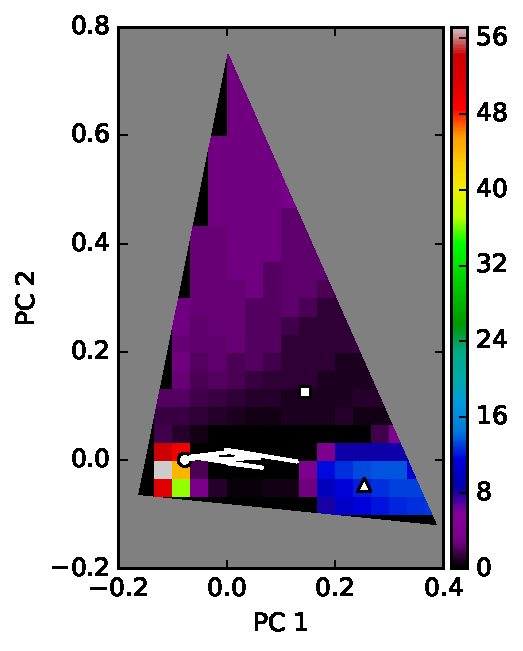
\includegraphics[width=\hsize]{IGBP_lon_noreg.pdf}
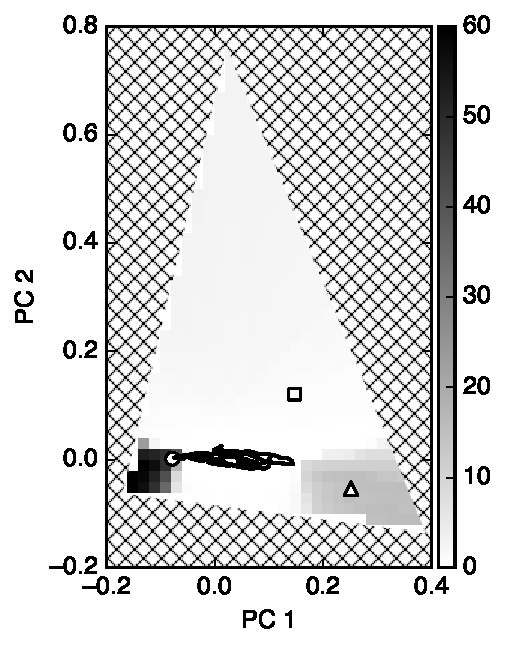
\includegraphics[width=\hsize]{IGBP_lon_noreg_allowedregion_gray.pdf}
    \end{center}
     \end{minipage}
    \caption{Upper panels: Probability of surface albedo spectra estimated from the light curves of $\alpha = 90^{\circ }$ (left), from the light curves of $\alpha = 135^{\circ }$ (middle) and from the colors of longitudinal slices. (Lower panels) Making the map coarser using HealPix. Left: 192 pixels, Middle: 48 pixels, Right: 12 pixels. }
\label{fig:PCplane}
\end{figure*}
%%%%%%%%%%%%%%%%%%%%%%%%%%%%%%%%%%%


Given that any three vertices in the principal component plane that enclose the trajectory/-ies can be a solution, the choice of the solution depends on the prior probability distribution. 
% Thus, we need to be careful about the implicit assumptions that are made  
With no assumptions or information on the spectral albedo of the surface types or geography, it is reasonable to assume that any points in the PC plane except for the inhibited regions are equally likely to correspond to a surface type. 
Despite this uninformative prior, the location of the light curve trajectory allows us to constrain the location of the surface spectra, in a probabilistic sense. 
%While such an assumption does not seem to work at all to choose the surface types, it does put some constrains. 
%While such an assumption does not uniquely specify the colors of all $K$ surface types, it does offer constraints due to the relative light curve trajectory within the permitted region. 
%This is because of the relative configuration of the trajectory and the permitted region. 
For example, in Figure \ref{fig:trajectory}, in order to enclose the trajectory with three surface types within the permitted region, we must have at least one point near the bottom left corner of the permitted region; this is consistent with the fact that one of the input albedo spectra (ocean) resides there. 

In order to see this more quantitatively, we make a grid on the PC plane  with an interval of 0.2 and consider all combinations of three grid points. 
Then, we assume that all of the combinations that enclose the trajectory are equally likely to be a solution, and find the marginalized probability of having a surface type at each location of the PC plane. 
Specifically, we consider the following Bayesian expression and attempt to find the posterior distribution:
%%%
\begin{equation}
P_{\rm posterior} ( t_{kn} | U_{in} ) = P ( U_{in} | t_{kn} ) \cdot P_{\rm prior} (  t_{kn} ) 
\end{equation}
%%%
where $t_{kn}$ represents the coordinates of the $k$-th surface type on the PC plane ($n$ is either 1 or 2, corresponding to PC 1 and PC 2), i.e., 
%%%
\begin{equation}
s_{kj} = \sum_n t_{kn} V_{nj} + \bar d_j . 
\end{equation}
Assuming that any location has the same prior probability per area of being a surface type, the prior for each $k$ is:
%%%
\begin{eqnarray}
&& P_{\rm prior} (t_{k1}, t_{k2} ) \, dt_{k1} dt_{k2} \\
&& = \left\{
\begin{array}{ll}
\displaystyle \frac{dt_{k1}  dt_{k2}}{\iint _{\rm allowed} d^2{\bf t}_k} & \;\;\;\;\;\; \mbox{if satisfies (\ref{eq:tilde_s_range})} \\
0 & \;\;\;\;\;\; \mbox{otherwise}
\end{array}
\right.
\end{eqnarray}
%%%
On the other hand, the likelihood is 
%%%
\begin{eqnarray}
&& P ( U_{in} | t_{kn} ) \\
&& \propto \left\{
\begin{array}{ll}
1 \;\;\; & \;\;\;\;\;\; \mbox{if satisfies (\ref{eq:tilde_f_range}) and (\ref{eq:tilde_f_range})} \\
0 \;\;\; & \;\;\;\;\;\; \mbox{otherwise}
\end{array}
\right.
\end{eqnarray}
%%%
Although the graphical meaning of conditions (\ref{eq:tilde_f_range}) and (\ref{eq:tilde_f_sum}) is simply to enclose the data, the judgement is numerically made \edit{by finding $\fast $ that satisfies condition (\ref{eq:tilde_f_sum}) from}\footnote{\edit{Note that the last matrix is a $K\times K$ matrix, and thus an inverse exists if $\{ {\bf t}_k \}$ forms a triangle (rather than a straight line or a single dot, in which case $\{ {\bf t}_k \}$ is not a solution anyways).}}
%%%
\begin{equation}
\begin{pmatrix}
U_{11} & U_{12} & 1 \\
... & & 1 \\
U_{I1} & U_{I2} & 1 
\end{pmatrix}
= 
\begin{pmatrix}
\fast_{11} & \fast_{12} & \fast_{13}  \\
... & \\
\fast_{I1} & \fast_{I2} & \fast_{I3}
\end{pmatrix}
\begin{pmatrix}
t_{11} & t_{12} & 1 \\
t_{21} & t_{22} & 1 \\
t_{31} & t_{32} & 1 
\end{pmatrix}
\end{equation}
%%%
or,
\begin{equation}
\begin{pmatrix}
\fast_{11} & \fast_{12} & \fast_{13}  \\
... & \\
\fast_{I1} & \fast_{I2} & \fast_{I3}
\end{pmatrix}
=
\begin{pmatrix}
U_{11} & U_{12} & 1 \\
... & & 1 \\
U_{I1} & U_{I2} & 1 
\end{pmatrix}
\begin{pmatrix}
t_{11} & t_{12} & 1 \\
t_{21} & t_{22} & 1 \\
t_{31} & t_{32} & 1 
\end{pmatrix}^{-1} 
\label{eq:f=ds-1}
\end{equation}
%%%
\edit{and asking if the resultant $\fast_{ik}$ are within the range of (\ref{eq:tilde_f_range}). }

Finally, we marginalize the posterior distribution, i.e.,
%%%
\begin{equation} 
P_{\rm posterior} ( {\bf t}_1) = \iint P_{\rm posterior} ( t_{kn} | d_{ij} ) d^2 {\bf t}_2 d^2 {\bf t}_3
\end{equation}
%%%
given the \edit{labeling degeneracy among} ${\bf t}_1$, ${\bf t}_2$, and ${\bf t}_3$. 
$P_{\rm posterior} ( {\bf t}_1) $ is normalized so that it sums up to unity. 

The resultant probability distribution is shown in Figure \ref{fig:PCplane}. 
As expected, we find a definite peak near the color of ocean. 
On the other hand, the peak that corresponds to \edit{sand} is a blur, and it is almost unconstrained. 
The vegetation in the bottom right corner is moderately constrained. 


%%%%%%%%%%%%%%%%%%%%%%%%%%%%%%%%%%%%%%%%%%%%%%%%%%%%%%%%%%%%%%
\subsection{Conditions for Successful Guess\\of Surface Spectra}
\label{ss:guess}
%%%%%%%%%%%%%%%%%%%%%%%%%%%%%%%%%%%%%%%%%%%%%%%%%%%%%%%%%%%%%%


We reiterate that in this framework the success of the surface retrieval critically depends on the relative configuration of the trajectory and the allowed region. 
More specifically, the good constraints on the colors of ocean appears to be due to the combination of the large covering fraction of ocean and the location of the color of ocean close to a corner in the PC plane (due to low albedo at longer wavelength). 

In order to illustrate these two effects and see under what conditions we can faithfully retrieve surface spectra, we created two additional mock light curves, (a) with the geographical maps of the \edit{sand} and vegetation being swapped, and  (b) with the geographical maps of the \edit{sand} and ocean being swapped. 
The left and right panels of Figure \ref{fig:swap} correspond to (a) and (b), respectively. 

%%%%%%%%%%%%%%%%%%%%%%%%%%%%%%%%%%%
\begin{figure}[htb!]
    \begin{center}
    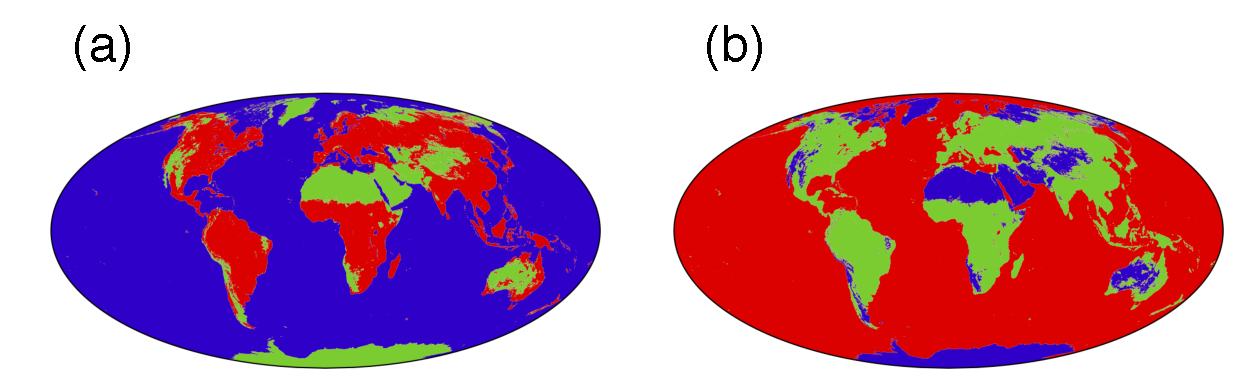
\includegraphics[width=\hsize]{swap_map.pdf}
    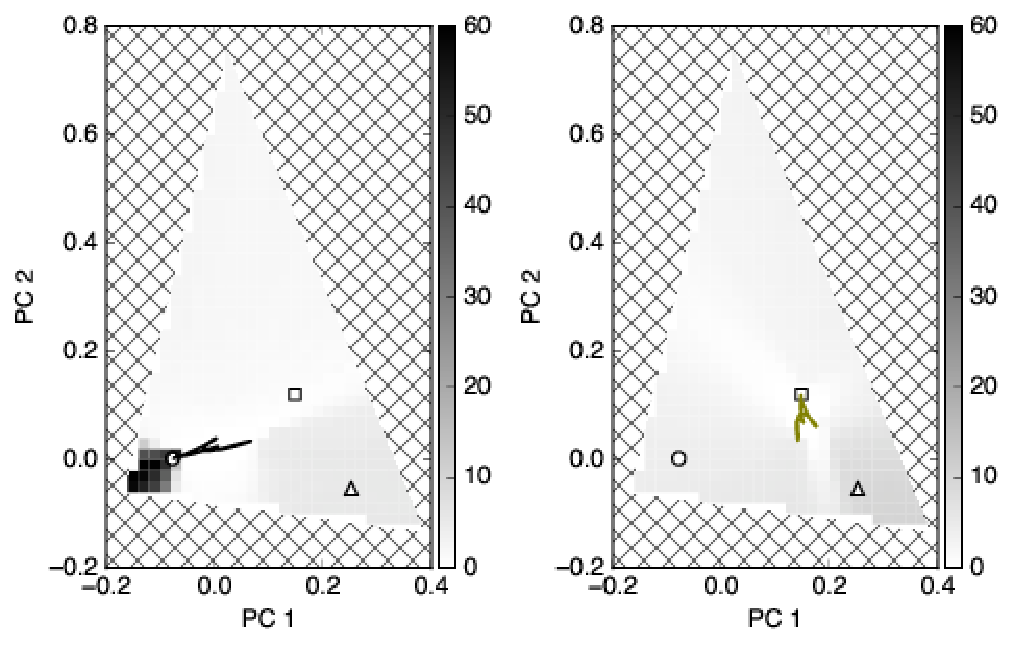
\includegraphics[width=\hsize]{mockdata_90deg_3types23_t360_lc_noreg_allowedregion_gray.pdf}
    \end{center}
    \caption{Left: Trajectory of the light curves with the geographical maps of the \edit{sand} and vegetation being swapped, and the resultant color contour of the posterior probability of albedo spectra of surface types. (b) Same as (a) but with the geographical maps of the \edit{sand} and ocean being swapped.}
\label{fig:swap}
\end{figure}
%%%%%%%%%%%%%%%%%%%%%%%%%%%%%%%%%%%

When we swap \edit{sand} and vegetation (left panel) the covering fraction of vegetation becomes smaller, and the trajectory of the light curves does not approach the vegetation endmember. As a result, the constraints on the color of vegetation become weaker. Thus, a large covering fraction of the surface type tends to yield a better constraint on the albedo spectra of that type; this agrees with our intuition.  

Meanwhile, in (b) we swap the \edit{sand} and ocean.  
Although \edit{sand} is now the dominant component, 
%the true location of the soil is rather not preferred based on 
our analysis prefers other locations toward the top of the allowed region, because there is more space there. 
Therefore, large covering fraction is not a sufficient condition for obtaining strong constraints on the color of a surface. 
\edit{Better constraints surface spectra can be obtained if its location on the PC plane is close to more than one boundaries of the allowed region. }
In other words, a surface spectrum can be well retrieved if it has favorable geography (ideally an entire hemisphere solely covered with that surface) {\it and} it has favorable albedo spectrum (albedo close to 0 or 1 at as many wavelengths as possible). 



%%%%%%%%%%%%%%%%%%%%%%%%%%%%%%%%%%%%%%%%%%%%%%%%%%%%%%%%%%%%%%
\section{Application to EPOXI data}
\label{s:EPOXI}
%%%%%%%%%%%%%%%%%%%%%%%%%%%%%%%%%%%%%%%%%%%%%%%%%%%%%%%%%%%%%%

%%%%%%%%%%%%%%%%%%%%%%%%%%%%%%%%%%%
\begin{figure}[tbh!]
    \begin{center}
	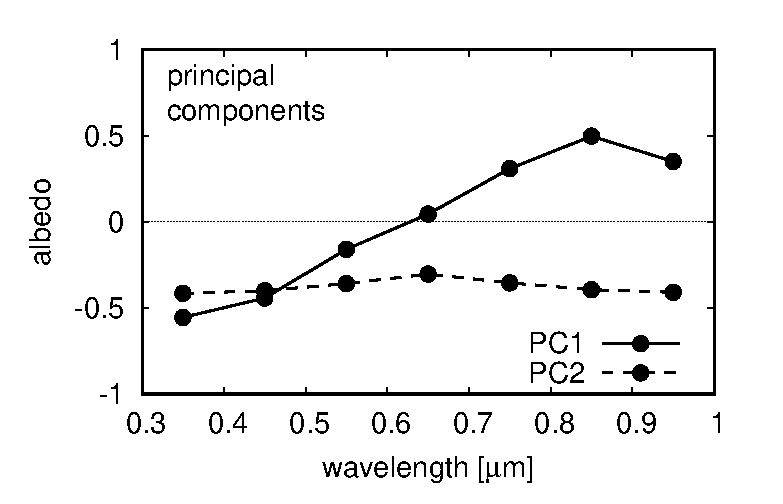
\includegraphics[width=0.85\hsize]{PCs_raddata_2_norm.eps}
	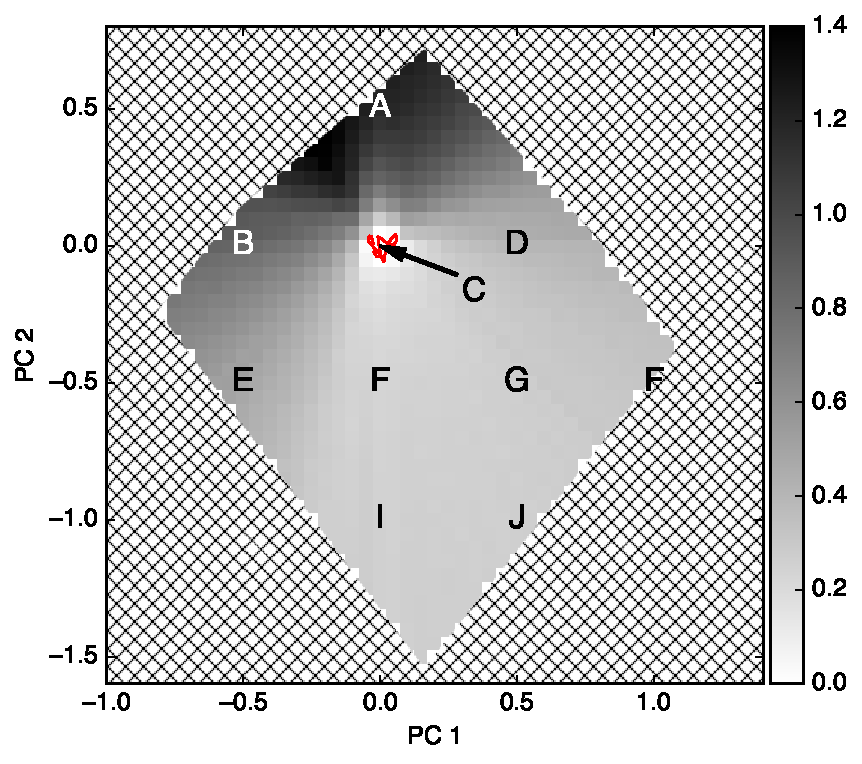
\includegraphics[width=0.88\hsize]{raddata_2_norm_noreg_ver2.pdf}
%	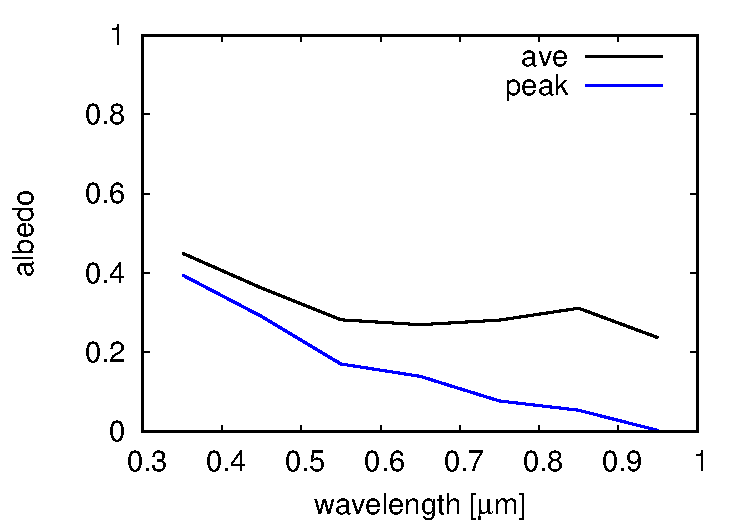
\includegraphics[width=\hsize]{raddata_2_norm_Mj_PCs.pdf}
	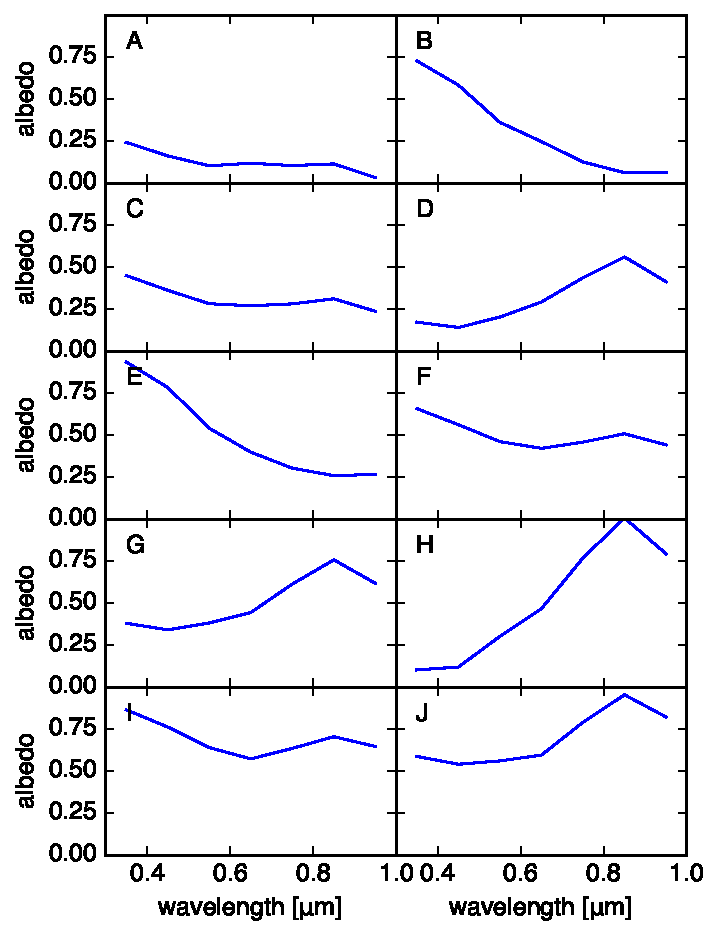
\includegraphics[width=0.85\hsize]{raddata_2_norm_spectra.pdf}
    \end{center}
    \caption{Top panel: PCs from EPOXI June data. Middel panel: color contour similar to Figure \ref{fig:PCplane}, but based on EPOXI observation of June 2008 \citep{Livengood2011}. The red line shows the light curve trajectory. Bottom panel: the spectra corresponding to the locations (A$\sim$J) shown in the upper panel. The ocean, \edit{sand}, and clouds appear to be close to A, D, and F, respectively. }
\label{fig:EPOXI}
\end{figure}
%%%%%%%%%%%%%%%%%%%%%%%%%%%%%%%%%%%



In this section, we apply our procedure to the observed multi-band light curves of Earth observed by the EPOXI mission. 
Specifically we use the same datasets as \citet{Cowan2013}, i.e., the 7-band diurnal light curves observed in June 2008 \citep{Livengood2011}. 
Using the two dominant PCs for these data, we performed the same analysis described in the previous section 

Figure \ref{fig:EPOXI} shows the trajectory of the light curve projected onto the PC plane, with the grayed region being the forbidden region. 
While the permitted region appears to be close to a square, it is in fact a heptagon, bounded by 7 inequalities (2\edit{-dimensional} slice through a 7\edit{-dimensional} hypercube). 
Overall, the upper boundaries come from the requirement of $s_{kj}>0$ while the lower boundaries comes from the requirement of $s_{kj}<1$. 

In this case, the trajectory of planetary color is far from the boundary because the color variations of the real Earth are muted by the cloud cover. 
Consequently, we do not see three peaks but a spectrum of the posterior probability distribution. 
Nevertheless, we are likely to find one surface type in the upper part of the allowed region, near label A \edit{, which can be interpreted as ocean}. 


%%%%%%%%%%%%%%%%%%%%%%%%%%%%%%%%%%%%%%%%%%%%%%%%%%%%%%%%%%%%%%
\section{Discussion}
\label{s:discussion}
%%%%%%%%%%%%%%%%%%%%%%%%%%%%%%%%%%%%%%%%%%%%%%%%%%%%%%%%%%%%%%

%%%%%%%%%%%%%%%%%%%%%%%%%%%%%%%%%%%%%%%%%%%%%%%%%%%%%%%%%%%%%%
\subsection{Confounding Factors}
\label{ss:confonting_factors}
%%%%%%%%%%%%%%%%%%%%%%%%%%%%%%%%%%%%%%%%%%%%%%%%%%%%%%%%%%%%%%


%%%%%%%%%%%%%%%%%%%%%%%%%%%%%%%%%%%%%%%%%%%%%%%%%%%%%%%%%%%%%%
\subsubsection{Uncertain Planetary Radius}

% So far we have assumed that the geometrical parameters are completely known, in particular, the planetary orbit, planetary spin axis and the planetary radius. 
% How would the uncertainties in these parameters affect our retrieval? 

So far, we have assumed that the data can be expressed in terms of apparent albedo. 
In reality, the primary observables from direct imaging observations are the intensities of the planet and the star. 
In order to convert them to the apparent albedo, we need to know the orbital distance from the star, the phase angle, and the planetary radius. 
While the former two can probably be constrained from multi-epoch observations, the radius continues to be severely degenerate with the planetary albedo. 
How would the unknown planetary radius affect our retrieval? 

Not knowing the planetary radius hence the normalization of the planetary albedo, we cannot put a tight upper limit on the surface albedo spectra, $s_{kj}$. 
%\memoYF{Possibly needs elaboration...please revise if you can explain better.} 
Thus, the condition (\ref{eq:tilde_s_range}) or (\ref{eq:s_range}) is virtually reduced to $0 \leq s_{kj}$. 
How much this limits our estimation depends on the configuration of PC plane in the $J$-dimensional space. 
For example, in the case of our mock data, the three significant constraints actually come from $0 \leq s_{kj}$ (see Figure \ref{fig:trajectory} and its caption), therefore the unknown normalization of planetary albedo does not affect the relative configuration between the light curves and the permitted region. 
Thus, the constraints of spectral shapes of the surfaces (but not the absolute scale) can be obtained. 
On the other hand, the case of EPOXI data would suffer from the unknown planetary radius, since roughly half of the boundaries of the permitted region originate from $ s_{kj} \leq 1$. 
In this case, our guess of the surface types would be deteriorated. 


%%%%%%%%%%%%%%%%%%%%%%%%%%%%%%%%%%%%%%%%%%%%%%%%%%%%%%%%%%%%%%
\subsubsection{Degenerate Dimensions in PC Plane}

The retrieval would become more complicated if \edit{the actual number of surface types is larger than the dimension of the PC plane plus 1 ($K > N + 1 $)}. 
For example, suppose the number of important surface types in EPOXI are actually four rather than three, which we cannot reject based on the data alone, then we would have to consider a tetragon to enclose all of the data points rather than a triangle. 
This affects our estimation of surface spectra. 
The greater the number of wavebands, the more improbable it is for multiple surface spectra to line on the same principle component hyperplane. 
Obtaining light curves in as many bands as possible will therefore help disentangle the surface colors in the $J$-dimensional band space. 


%%%%%%%%%%%%%%%%%%%%%%%%%%%%%%%%%%%%%%%%%%%%%%%%%%%%%%%%%%%%%%
\subsubsection{Deviation from Lambert's Law}
\label{ss:deviate_Lambert}

We have assumed that the surface scattering obeys Lambert's law, but in reality they are not perfect Lambert scatterers. 
In particular, scattering by ocean exhibits prominent specular reflection and the reflectivity increases when the incident light is grazing, or equivalently at crescent phase \citep[e.g.,][]{Williams2008,Robinson2010,Robinson2014}. 
Furthermore, when we take account of an atmosphere above the surface, the albedo spectra of surface overlaid by an atmosphere changes with phase angle.  
Considering these effects, the trajectories of the light curves at different phases do not have to reside in the same PC plane. 
These light curves can be analyzed independently, and the components varying with phase would give us insights into the anisotropic scatterers. 




%%%%%%%%%%%%%%%%%%%%%%%%%%%%%%%%%%%%%%%%%%%%%%%%%%%%%%%%%%%%%%
\subsection{Enhancing Constraints}
\label{ss:enhancing_constraints}
%%%%%%%%%%%%%%%%%%%%%%%%%%%%%%%%%%%%%%%%%%%%%%%%%%%%%%%%%%%%%%


%%%%%%%%%%%%%%%%%%%%%%%%%%%%%%%%%%%%%%%%%%%%%%%%%%%%%%%%%%%%%%
\subsubsection{Power of Many Bands}

%\memoYF{What do you think about this subsection? I thought we could include this in conclusion and abstract. }

As we discussed Section \ref{ss:guess}, the constraints on the surface spectra rely on the relative configuration between the light curve trajectories and the boundaries of the physically permitted region, namely that albedo of any surface must be between 0 and 1 at all wavelengths. 
It depends on geography and the albedo spectra of the surface types, neither of which we can directly change. 
However, we can potentially increase the number of boundaries of the permitted region by increasing the number of photometric bands, and some of them may have tighter constraints than others. 
Observing the light curves in as many bands as possible will therefore be beneficial.  
In particular, observing at wavelengths where one or more surface types have albedo close to 0 or 1 \edit{constrain the possible albedo more tightly}. 
Albedo closer to 0 (i.e., the condition of $0 \le s_{kj}$) are more useful because it does not depend on the uncertainties in the radius. 
In reality, albedo of ocean is close to 0 at longer wavelength toward near infrared, that of \edit{sand} is small at 0.4 $\mu $m and shortward, that of vegetation is close to 0 at 0.7 $\mu$m and shortward, and that of H$_2$O snow is close to 1 in the visible and closer to 0 at 1.5 $\mu$m and 2 $\mu$m bands. 
Observations at different bands covering these characteristic wavelengths would be useful. 
% Conversely, surfaces overlaid with clouds have muted spectral features with higher albedo than the bare surfaces, which would make the retrieval more challenging. 

%%%%%%%%%%%%%%%%%%%%%%%%%%%%%%%%%%%
\begin{figure*}[hbt!]
   \begin{minipage}{0.33\hsize}
    \begin{center}
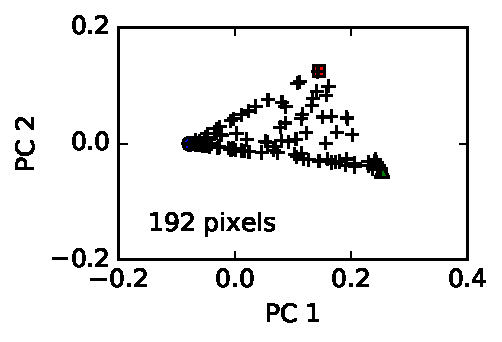
\includegraphics[width=\hsize]{IGBP_PCplane_Nside2.pdf}
    \end{center}
     \end{minipage}   
    \begin{minipage}{0.33\hsize}
    \begin{center}
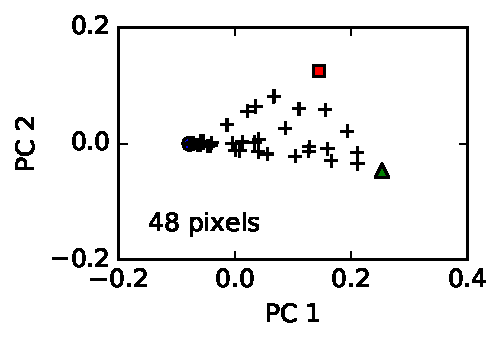
\includegraphics[width=\hsize]{IGBP_PCplane_Nside1.pdf}
    \end{center}
     \end{minipage}
   \begin{minipage}{0.33\hsize}
    \begin{center}
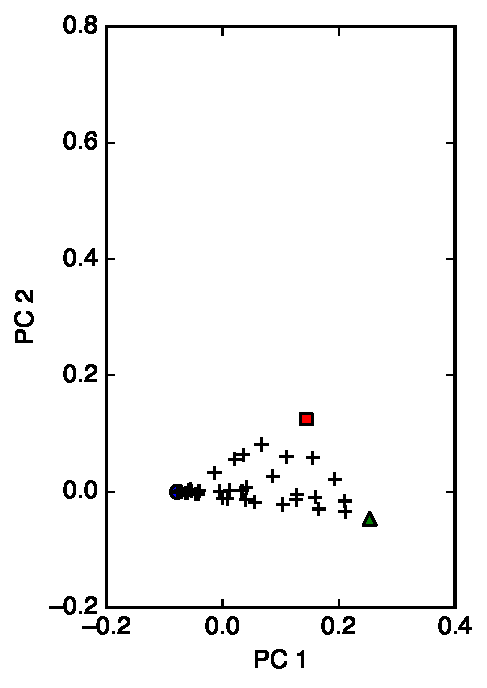
\includegraphics[width=\hsize]{IGBP_PCplane_Nside0.pdf}
    \end{center}
     \end{minipage}
    \caption{Making the map coarser using HealPix. Left: 192 pixels, Middle: 48 pixels, Right: 12 pixels. }
\label{fig:lowresolution}
\end{figure*}
%%%%%%%%%%%%%%%%%%%%%%%%%%%%%%%%%%%


%%%%%%%%%%%%%%%%%%%%%%%%%%%%%%%%%%%%%%%%%%%%%%%%%%%%%%%%%%%%%%
\subsubsection{Utilizing Light Curves at Different Phases}



Light curves at different orbital phases are useful in spectral unmixing, because they shed light on different locations on the surface with varying weight, exploring the PC plane in different directions. 
As a result, the volume of color space where the solution can exist will be narrowed.  
In particular, the diurnal light curves at thinner phase tend to exhibit larger color variations, giving tighter constraints (but see the caveat in Section \ref{ss:deviate_Lambert}). 

In addition, diurnal light curves at different orbital phases in principle allow us to map the color in 2 dimensions.   \citep{Kawahara2010,Kawahara2011,Fujii2012}. 
We could then use the mapped spectra (spectra of various surface patches resolved in 2 dimensions) to identify different surface types, in the same spirit as that of estimating the covering fraction of longitudinal slices $f_{lk}$ and $s_{kj}$ . 
In fact, this ``map first'' approach is likely more appropriate with 2-dimensional maps than with longitudinal maps for the following reason. 
In the diurnal light curves at a single phase, colors of very distant pixels beyond the correlation length of the geography are mixed together, even at crescent phases---for example, the colors of the arctic, tropics, and antarctic are mixed in an equatorial observation, no matter how extreme the orbital phase is. 
As a result, the colors of longitudinal slices never approach the colors of vegetation or \edit{sand} despite the number of slices, as shown in the right panel of Figure \ref{fig:PCplane}. 
The situation is different when we gradually lower the resolution of the 2-dimensional maps. 
Figure \ref{fig:lowresolution} shows the colors of HEALPix pixels \citep{Gorski2005} with varying resolutions: from left to right, we change the resolution from 192 pixels, 48 pixels to 12 pixels, starting from the map in Figure \ref{fig:mockdata}. 
The triangular shape of the locus of points becomes apparent with as low resolution as 48 pixels. 
Thus, resolving the surface colors in 2 dimensions will ease our challenge to identify the surface types. 



%%%%%%%%%%%%%%%%%%%%%%%%%%%%%%%%%%%%%%%%%%%%%%%%%%%%%%%%%%%%%%
\subsubsection{Invoking Additional Assumptions}

Occasionally, we may want to adopt additional constraints on the behavior of $\fast _{ik}$ ($f_{lk}$) or $s_{kj}$ based on the prior assumptions. 

For example, we may assume that the covering fractions of surface types  ``smoothly'' vary as a function of time or longitude. 
Such an assumption could be implemented via a Gaussian Process \citep[e.g.,][]{Rasmussen2005}, i.e., the area fractions at different times/longitudes have joint gaussian distribution with the relevant correlation length. 
We must exercise because the actual covering fractions of surface types are not necessarily a Gaussian Process. 
%In our mock data, ocean appears to be better approximated by Gaussian Processes than vegetation and soil. 
\edit{\sout{As a result, imposing Gaussian Process tends to yield better estimation of ocean color and biased estimation of \edit{sand} color. }[YF: removed because it is hard to understand without more detailed description, which I doubt needs here.]}

We could also consider a regularization on albedo spectra as a function of wavelength. 
This can be regarded as a prior probability distribution on the PC plane. 
For example, in Figure \ref{fig:PCplane}, albedo spectra corresponding to the upper part of the permitted region exhibit a dramatic decrease in albedo between 0.65$\mu $m and $0.75\mu $m, which we may seem implausible. 
However, such constraints are based upon our prior assumptions and may not be true. 
Albedo spectra of vegetation in fact have a sharp feature, the red edge, and similar, unfamiliar features may exist on other planets. 
In addition, with an atmosphere, absorption by atmospheric molecules can also produce sharp changes in albedo spectra. 


%%%%%%%%%%%%%%%%%%%%%%%%%%%%%%%%%%%%%%%%%%%%%%%%%%%%%%%%%%%%%%
\section{Summary}
\label{s:conclusion}
%%%%%%%%%%%%%%%%%%%%%%%%%%%%%%%%%%%%%%%%%%%%%%%%%%%%%%%%%%%%%%

In this paper, we revisited the problem of estimating the albedo spectra of major surface type and their distribution\edit{s} from disk-integrated \edit{colors} of exoplanets. 
We pointed out the inherit degeneracy which makes it impossible to find unique solutions. 
Despite the degeneracy, \edit{the following physical conditions narrow down the possible  solutions for the surface albedos:
the actual surface albedo spectra in the $J$-dimensional color space are (1) to be located on the PC (hyper-)plane, (2) to enclose all of the data points of the disk-integrated colors, and (3) to be in the $J$-dimensional hypercube, bounded by 0 and 1 for all axes. %
We demonstrated using both a simplified toy model of Earth and the observed data by EPOXI that such constraints point us to the approximate spectra of ocean. }

\edit{In more general, we find that the success of the estimates critically depends on the degree of excursions of the trajectory of the disk-integrated colors, and its orientation in the color space.  %
In other words, the estimates will be better if the covering fraction of each surface type becomes close to 1, as an intuition suggests. 
In addition, observations at the many wavelengths where surface albedo are close to 0 or 1 could improve the estimates. }
\edit{As the wavelength coverage/resolution increases, and as the light curves at more orbital phases are obtained, the performance of our procedure will be refined. [YF: too obvious??]}


\acknowledgements

We acknowledge the Exo-Cartography workshops supported by the International Space Science Institute (ISSI). 
Y. F. acknowledges the generous support from Universities Space Research Association through an appointment to the NASA Postdoctoral Program at the NASA Goddard Institute for Space Studies. 
Y. F. also acknowledges support from the NASA Astrobiology Program through the Nexus for Exoplanet System Science. 
J.~L.~Y. is supported by the NASA Astrobiology Institute's Virtual Planetary Laboratory under Cooperative Agreement number NNA13AA93A. 
N.~B.~C. is supported by the McGill Space Institute and Institut de recherche sur les exoplan\'etes.  

\bibliography{ref}

\end{document}